\chapter{Introduction}
\label{cha:Introduction}

Computational efficiency of algorithms have reached almost a peak over the years
and further improvements using system level parallelism such as multiprocessing, multi-core systems
or instruction level parallelism such as pipelining etc. has also not proven to significantly contribute
towards further improvement. These limitations have led to use of parallel multi-core processing
systems which use multiple CPUs, GPUs and FPGAs to speed up the processing of applications
which require high computational performance. These systems, generally referred as supercomputers or
high performance clusters, comprises of multiple individual systems known as nodes. Each node
can contain multiple multi-core processing, GPUs and FPGAs and are connected to each other
using high speed Ethernet to exchange data and control information. The whole system acts
as a single high performance system with distributed memory and processing elements as
shown in figure \ref{fig:cluster}

\begin{figure}[ht]%
    \centering
    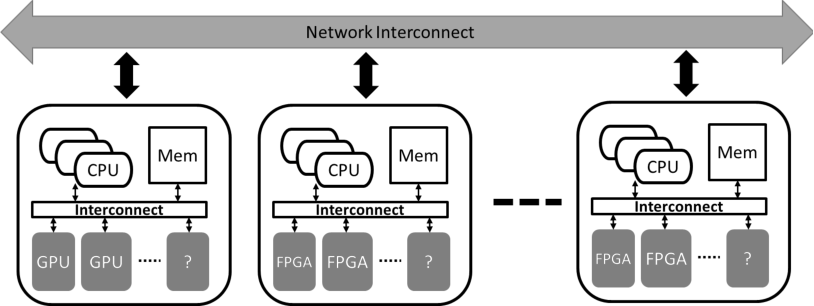
\includegraphics[width=1.0\textwidth]{images/cluster}
    \caption{High performance cluster structure with multiple nodes having different configuration}
    \label{fig:cluster}
\end{figure}

Traditionally multiple CPU based supercomputers were only utilized but considering the nature
of the application which mostly consists of the same operation performed on a stream of data,
GPUs which could do multiple of these operations in parallel \ac{SIMD} were utilized
to increase performance further. The GPUs act as accelerators and are attached to main CPUs
which offloads vector based computation suitable for GPU via special software constructs.
The GPUs help in reducing a lot of computation time for large amount of data.Though the CPU
and GPU based parallel architecture provide significant performance benefits,
these are limited by the size of the cluster and the problem size. These limitations led
researchers to look for technologies which would help in decreasing the execution time for
single step even further by using hardware based accelerators.

FPGA based accelerators are thus seen as the most prominent alternative. FPGAs provide the flexibility
to design application specific hardware accelerators and re-use the same FPGA for different kinds
of problem without huge programming overheads. FPGAs as an accelerator is mostly used to implement
simple mathematical operations such as matrix multiplication, fast fourier transformation and
string manipulation which form the basis for most of the application. Using the FPGA's features
such as data and instruction pipelining, replication and memory localization, the FPGAs can be
used to decrease the execution time of these mathematical operations.

Increasing popularity of the FPGAs in the high performance computing has led to new innovations for
the FPGAs. Higher memory bandwidths, increased count of logical units and bigger local memory
are some of these. The new Noctua \ac{HPC} cluster at Paderborn Center for Parallel
Computing (PC\textsuperscript{2}) contains the current generation of Intel Stratrix 10 FPGAs which provide
specialized high speed serial IO channels which can be used to set up communication infrastructure
between the FPGAs. The BittWare 520N boards used are equipped with four 100/40/25/10G
QSFP28 network ports which use these serial IO channels and would provide a very high speed
communication setup and opportunities to scale up application over multiple FPGAs with small
communication latency replacing applications which use MPI for communication.

MIDG2\footnote{\url{https://github.com/tcew/MIDG2}} is an MPI based parallel computation
implementation of the \ac{DG} \cite{hesthaven_nodal_2008} method to solve Maxwell’s equation
in time domain. \ac{DG} method is a commonly used operation in many simulation applications to
solve \ac{PDE} and improvements to the computation time would be an important step to
benefit different simulation applications utilizing this method. This thesis presents
a design which evaluates the benefits of using a parallel distributed FPGA based system
to reduce the execution time of the application by using direct FPGA-to-FPGA communication.

\section{Objectives}

The Noctua being first of the academic \ac{HPC} cluster equipped with FPGAs provides
opportunities to create systems which are accelerated with multiple FPGAs. As there is
no known implementation utilizing FPGA in network configuration for accelerating the
DG method, this master thesis aims at presenting such a system to evaluate
the achievable acceleration with multiple FPGAs using point-to-point communication in
different network topologies for the MIDG2 application. Towards achieving this target,
the evaluation can be divided into two stages. First stage aims at identifying
and evaluating the possible topologies for point-to-point communication. In the second
stage of the thesis, the existing openCL™ based FPGA implementation for
the MIDG2 application would be extended to use IO channels.

Considering the two stages as individual sub-tasks, the first task involves building
prototypes using openCL™ IO channels which would utilize the four 100/40/25/10G QSFP28
network ports available on the BittWare 520N boards. These prototypes would be used
to evaluate the point-to-point topologies using bandwidths and latency to give an
overview of possible benefits. The prototypes would also serve as the basis for
understanding the implementation opportunities available in the openCL™ and
BittWare BSP for the channels. The second task would be then to utilize the
understanding and extend the openCL™ kernels for the MIDG2 application
such that the need for MPI communication to communicate information or the shared
surfaces is eliminated and overheads involved the removed.


\section{Related Work}

\ac{DG} method is believed to be first proposed by \textcite{reed_triangular_1973} for
solving the steady-state neutron transport equation \cite{hesthaven_nodal_2008}. Over the
years many researchers have proven the accuracy of the method and developed improvements
over the original method to use in different fields for solving \ac{PDE}. The \ac{DG} method
is popular today to solve equations in the fields of acoustics \cite{wilcox_high-order_2010,
atkins_quadrature-free_1998, toulopoulos_high-order_2006}, elasticity \cite{dumbser_arbitrary_2006,
kaser_arbitrary_2006, kaser_arbitrary_2007}, electrodynamics Maxwell’s equation \cite{busch_discontinuous_2011,
cohen_discontinuous_2006, busch_discontinuous_2011, cohen_spatial_2006, cockburn_locally_2004,
konig_discontinuous_2010} and thermodynamics \cite{collis_discontinuous_2002}.

The popularity of the \ac{DG} method has led researchers to develop parallel methods
which can speed up the application to reduce the execution time. As the DG method
performs operations on local elements followed by accumulation, this allows parallelization
of the operations on elements and has been utilized to create various parallel systems.
\textcite{baggag_parallel_1999} presents a parallel system which is used to simulate aeroacoustic
scattering and uses MPI data exchange. \textcite{klockner_nodal_2009} showed the benefits
of using GPU for accelerating the computation by utilizing the capability of the GPU to
process data in parallel. They use CUDA programming for GPUs to get improved memory bandwidths
and higher computation efficiency. \textcite{bernacki_parallel_2006} discuss the benefits
of parallelization achieved by partitioning the tetrahedral meshes for realistic problems
involving electromagnetic wave radiation study for different objects. Though the use of such
parallel architecture and use of GPU based accelerators have proven
to improve the simulation time, they often require large data sets to show the benefits of
such improvements.

FPGAs based accelerators allows to overcome such issue as they provide architecture
such as efficient arithmetic operations using DSPs, deep instruction and pipelining
to decrease computation time, replication for large scale parallel computations.
Such benefits have made FPGAs a popular choice for implementing accelerators for
problems utilizing heavy floating point computation. Considering such benefits,
an implementation for accelerating the \ac{DG} operations in FPGAs was
developed by \textcite{kenter_opencl-based_2018}. The implementation shows the benefit
of using a single FPGA over a highly parallelized multi-core CPU implementation for
the MIDG2 application which solves Maxwell’s equations in time domain. An extension
of this design is implemented by PC2 which is capable or using multiple FPGAs using MPI.
This design is used as the base for this thesis.

The increased popularity of the FPGAs in past as led to identify possibilities for
using multiple FPGAs. This can be achieved by using MPI communication via the host
to which the FPGA is connected. Though such design posses benefits in many cases,
it performs poorly in case of multiple and large transfer due to very low bandwidths
for the PCIe + MPI combination. Systems have been investigated where the FPGAs could
communicate directly without the need of host. \textcite{sheng_hpc_2017} presents a design
for 3D FFT solver which uses a 3D-torus FPGA-based network using a table-based routing
scheme. The evaluation results of such design shows 30\% improvement over the reference design.
\textcite{kobayashi_opencl-ready_2018} used an openCL™ based design implementation to
compare the latency of MPI+PCIe based system and FPGA-to-FPGA system which uses Ethernet
IP for communication over an switch. The results show a large difference between the achievable
bandwidths and latency for the two system proving the benefits of such system. The system
design presented in this thesis uses a similar approach like in \cite{kobayashi_opencl-ready_2018}
but does not utilize the Ethernet-IP core and relies on the serial communication
support provided in the BittWare BSP.

The rest of the thesis is divided into 5 chapters. Chapter \ref{cha:Fundamentals} would
discuss the fundamentals of the components and technologies used in the thesis.
Chapter \ref{cha:topologies} introduce the topologies which are possible for the FPGAs
along with the prototypes developed for the evaluation. Chapter \ref{cha:sys_arch}
explains the first implementation done using IO channels. Chapter \ref{cha:sys_fpgaonly}
presents the FPGA only system implemented by optimizing the IO channels design
to remove the host dependency in the kernels. Chapter \ref{cha:Evaluation} discusses the evaluation steps
and the results of the evaluation in detail highlighting the benefits of using the IO channels.
Final chapter \ref{cha:Conclusion} presents a conclusion of the achieved results of the thesis
and proposes possible future works and improvements.